\documentclass{tufte-handout}

\title{Leafleting Effectiveness Survey (LES)}
\author[Jack Norris \& Eric Roberts \& Jonathon Smith]{Jack Norris\thanks{Executive Director, Vegan Outreach} \& Eric Roberts\thanks{Research Manager, California Department of Health Services} \& Jonathon Smith\thanks{Technical Group Supervisor, Jet Propulsion Laboratory}}

\date{June 2017} % without \date command, current date is supplied
%\geometry{showframe} % display margins for debugging page layout

\usepackage{graphicx} % allow embedded images
  \setkeys{Gin}{width=\linewidth,totalheight=\textheight,keepaspectratio}
  \graphicspath{{graphics/}} % set of paths to search for images
\usepackage{amsmath}  % extended mathematics
\usepackage{booktabs} % book-quality tables
\usepackage{units}    % non-stacked fractions and better unit spacing
\usepackage{multicol} % multiple column layout facilities
\usepackage{colortbl}   % filler text
\usepackage{fancyvrb} % extended verbatim environments
\usepackage[export]{adjustbox}

  \fvset{fontsize=\normalsize}% default font size for fancy-verbatim environments

% Standardize command font styles and environments
\newcommand{\doccmd}[1]{\texttt{\textbackslash#1}}% command name -- adds backslash automatically
\newcommand{\docopt}[1]{\ensuremath{\langle}\textrm{\textit{#1}}\ensuremath{\rangle}}% optional command argument
\newcommand{\docarg}[1]{\textrm{\textit{#1}}}% (required) command argument
\newcommand{\docenv}[1]{\textsf{#1}}% environment name
\newcommand{\docpkg}[1]{\texttt{#1}}% package name
\newcommand{\doccls}[1]{\texttt{#1}}% document class name
\newcommand{\docclsopt}[1]{\texttt{#1}}% document class option name
\newenvironment{docspec}{\begin{quote}\noindent}{\end{quote}}% command specification environment

%\newcommand{\sitslong}[0]{\textsc{Spacecraft In The Shot}}% document class option name
\newcommand{\les}[0]{\textsc{LES}}% document class option name
\newcommand{\totalbooklets}[0]{\textsc{130000}}% document class option name                  
\newcommand{\stickercost}[0]{\textsc{22500}}% document class option name                  
\newcommand{\giftcardnum}[0]{\textsc{9000}}                                   
\newcommand{\giftcardcost}[0]{\textsc{67500}}
\newcommand{\schoolnum}[0]{\textsc{90}}

\begin{document}

\maketitle% this prints the handout title, author, and date

%\begin{itemize}
%\color{red}
%    \item Name of submitter and contact information (institutional affiliation, email address, phone number).
%    \item SMD research discipline with which the suggested new science investigation is best aligned (Astrophysics, Earth Science, Heliophysics, or Planetary	Science)
%    \item Desired orbit locations including any launch window constraints;
%\end{itemize}

% ---------------------------------------
% ---------------------------------------
\begin{abstract}
\noindent

Near the beginning of Fall semester 2017, a total of \totalbooklets~ 
students will be handed a leaflet. Half the leaflets will have a
pro animal rights message (\textbf{test books}), half will be on a
non-animal related topic (\textbf{control books}). Each booklet will have a
sticker advertising a ``\$5 Starbucks or Amazon Gift Card for taking
brief survey" (\textbf{Part 1 Survey}). Students answering the survey will be 
asked about their current consumption of animal products (\textbf{base rate}) 
and given a gift card. Two months later, just before Thanksgiving 
break, these same students will receive an email, "Thanks for taking 
our previous survey! We have a few more questions, of course for 
another \$10 gift card!" (\textbf{Part 2 Survey}). Students will again
be asked about their current animal consumption. The data will
be examined to see if the pro-animal leaflets reduce the amount of
animal products consumed by the students (\textbf{post-test rate}), 
particularly to zero (the \textbf{``One Week Vegan"}). 

\end{abstract}

\begin{marginfigure}[-2 in]%
  \raggedleft
  
\includegraphics[width=\textwidth]{vologo.png}
  \caption{Vegan Outreach was founded in 1993 and has since handed out more
  than 30 million pro-vegetarian leaflets. They are the organization leading 
  the proposed LES Study.}
  \label{fig:vologo}
\end{marginfigure}

%\begin{marginfigure}[0 in]%
%  \includegraphics[width=\textwidth]{sitsdepiction.png}\\
%  \includegraphics[width=.98\textwidth]{sitsdepiction2.png}
%  \caption{Illustration of a \sitsshort~ Imager capturing footage of 
%           Jupiter Orbit Insertion burn. After collection, the imager 
%           is left behind.}
%  \label{fig:sitsdepiction}
%\end{marginfigure}
  
\newthought{The Leafleting Effectiveness Survery (\les)} will attempt
to quantify the impact of pro-animal leafleting on the later 
consumption of animal products. In particular it will look for 
``one week vegans", or leaflet recipients who report no consumption of animal 
products in the post-test survey week. 
The relationship between leafleting and one week vegans is of real
concern for the organization leading \les, Vegan Outreach (VO). VO's
primary intervention on behalf of animals is to hand out pro-vegetarian,
anti-speciest literature to college students. Verifying the impact of this
intervention has become an organizational priority at the highest level.
VO also understands that this is a general concern of the broader
animal protection community, and has sought the support and advice of
partner organizations to carry out \les.

In particular, VO seeking the participation of Animal Charity 
Evaluators (ACE) as a partner on \les. This document outlines VO's formal
request for a grant from ACE's Animal Advocacy Research Fund. VO is 
looking to ACE to finance (1) the printing of \totalbooklets~ 
survey-advertising stickers (\$\stickercost) (2) the purchase of
\giftcardnum~ gift cards to distribute as incentives for taking the 
survery (\$\giftcardcost), and (3) the creation of a public website
to share the results (\$\websitecost).

\begin{fullwidth}
{
\fontsize{9pt}{9pt}\selectfont
\vskip 1.5em
\noindent
\textsc{\les~ At A Glance}
\noindent
\begin{itemize}
    \item[] Utilizes a pre- and post- survey to measure the 
            impact of leafleting on self-reported animal product 
            consumption.
    \item[] Pilot studies indicate that a brightly colored sticker 
            attached to leaflets advertising an incentivized survey
            (\$5 for P1, \$10 for P2, \$15 total per participant) can 
            generate a response rate of roughly 5\%.
    \item[] A total of \totalbooklets~ will be handed out (half test, 
            half-control), powering the study to detect a conversion of
            1\% or greater of the test population into a one week vegan.
    \item[] The leaflets will be handed out at \schoolnum~ schools in
            September 2017. Recipients have one week after the leaflets
            are handed out to complete the Part 1 survey. An email will
            be sent out to students who completed Part 1 in 
            mid-November, inviting them to fill out the Part 2 survey.
\end{itemize}
}
\end{fullwidth}

% ---------------------------------------
% ---------------------------------------
\section{Background}\label{sec:background}

\begin{itemize}
\color{red}
    \item Talk here about previous leafleting studies
    \item Talk here about pilot studies.
\end{itemize}

\newthought{Vegan Outreach} has run a total of three pilot studies
in preparation for a full-scale LES. These pilots have focused primarily on 
crafting a study approach that results in a sufficiently high survey response rate to
make a fully powered LES tractable. The current study design (brightly colored stickers 
and \$15 incentive for 5\% response rate) is a direct result of these studies, summarized 
below.  

\begin{fullwidth}
{  
\fontsize{9pt}{9pt}\selectfont
\vskip 1.5em
\noindent
\textsc{LES Pilot Studies}
\vskip 1em
\noindent
Pilot 1: Fall 2015 
\begin{itemize}
  \item[] The first pilot study utilized a test group of 5000 and a control group of 1000. 
  \item[] Plain white stickers advertised a \$5 incentivized survery.
  \item[] Overall response rate (P1 \& P2) was 1.88\%. 
\end{itemize}
\noindent 
Pilot 2: Spring 2016 
\begin{itemize}
  \item[] Two tests groups were used both with 100 participants.  
  \item[] Plain white stickers advertised \$10 (group 1) and \$20 (group 2) incentivized surveys.
  \item[] Response rates were 3\% and 2\% respectively. 
\end{itemize}
Pilot 3: Spring 2016 
\begin{itemize}
  \item[] Test group with 600 participants.  
  \item[] Colored stickers advertised a \$5 incentivized survey. 
  \item[] An additional \$10 was offered to complete Part 2 of the survey.
  \item[] Response rate was 5\%. 
\end{itemize}
\vskip 1.5em
}
\end{fullwidth}

\begin{marginfigure}[-5 in]%
  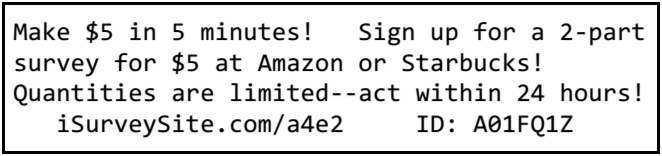
\includegraphics[width=\textwidth]{les_sticker_1.png}\\
  
\includegraphics[width=.98\textwidth]{les_sticker_2.png}
  \caption{Stickers used to adeverstise incentivised surves, pilot 1 and 2 (top), pilot 3 (bottom).}
  \label{fig:lesstickers}
\end{marginfigure}

The full-scale LES will use the strategy from Pilot 3. The key elements are
(1) colored stickers, (2) \$5 incentive for Part 1 survey, (3) \$10 for Part 2
survey. d

\begin{marginfigure}[-1 in]%
  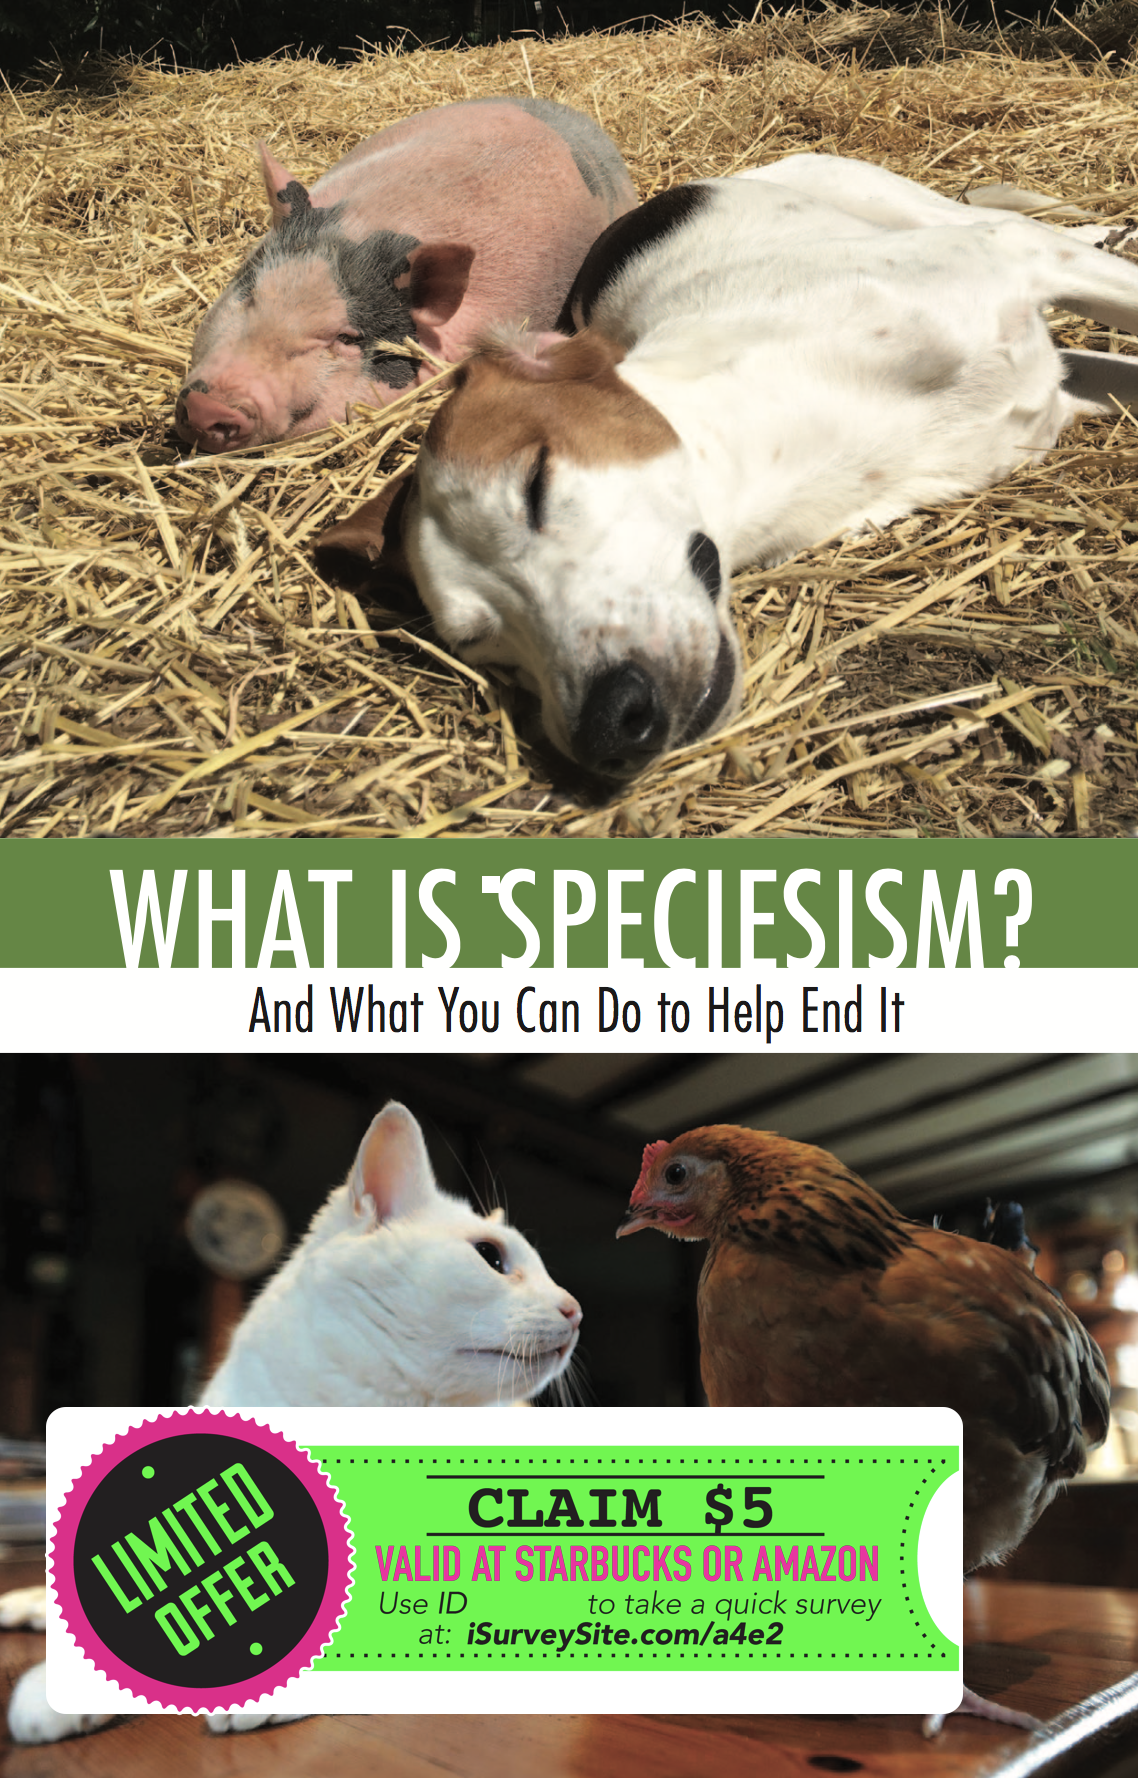
\includegraphics[width=\textwidth]{les_booklet_mockup.png}
  \caption{Mockup of test booklet with survey sticker.}
  \label{fig:lesbooklet}
\end{marginfigure}

% ---------------------------------------
% ---------------------------------------
\section{Parameters}

\begin{itemize}
\color{red}
    \item Put the relevant power calculations in here.  	
\end{itemize}



% ---------------------------------------
% ---------------------------------------
\section{Plan and Budget}

\begin{itemize}
\color{red}
    \item Outline the study plan (partners, schedule, etc)
    \item Put in full study budget.  	
\end{itemize}

\begin{fullwidth}
{
\fontsize{9pt}{9pt}\selectfont
\vskip 1.5em
\noindent
\textsc{\les~ Study Timeline}
\noindent
\begin{itemize}
    \item[\textbf{Aug  14}] Ship test / control booklets and stickers to leafleters.
    \item[\textbf{Aug  28}] Complete applying stickers to booklets.
    \item[\textbf{Sep  5}] Begin handing out booklets                           
    \item[\textbf{Sep 19}] Complete handing out leaflets 
    \item[\textbf{Sep 25}] Close Part 1 survey 
    \item[\textbf{Nov 11}] Send invitations for Part 2 survey 
    \item[\textbf{Nov 18}] Close Part 2 survey. 
\end{itemize}
}
\end{fullwidth}


\begin{table*}
  \fontfamily{ppl}\selectfont
  \begin{tabular}{lll}
    \toprule
    Category  & Cost & Partner \\
    \midrule
    
    Attaching stickers  & 22500.0 & Vegan Outreach\\                
    
    Leafleting (Small School)  & 4500.0 & Vegan Outreach\\                
    
    Leafleting (Large School)  & 4500.0 & Humane League\\                
    
    \midrule
                               
    Test Booklets  & 5250.0 & Vegan Outreach\\                                    
                               
    Control Booklets  & 5250.0 & Vegan Outreach\\                                    
                               
    Stickers  & 22500.0 & ACE\\                                    
         
    \midrule
                               
    Gift Cards  & 67500.0 & ACE\\                                    
         
    \bottomrule
  \end{tabular}
  \vskip 1.5em
  \caption{Detailed \les~ Budget}
  \label{tab:budget}
\end{table*}

% ---------------------------------------
% ---------------------------------------
%\section{Closing Thoughts}\label{sec:close}


\end{document}  
